\documentclass[handout]{beamer}
\usepackage[utf8]{inputenc}
\usepackage[T2A]{fontenc}
\usepackage[english]{babel}
\usepackage{graphicx}
\usepackage{array}
\usetheme{Warsaw}
\usecolortheme{wolverine}

\usepackage{fontawesome5}
\usepackage{listings}
\usepackage[all]{xy}
\usepackage{changepage}

\definecolor{dkgreen}{rgb}{0,0.6,0}
\definecolor{gray}{rgb}{0.5,0.5,0.5}
\definecolor{mauve}{rgb}{0.58,0,0.82}

\lstdefinelanguage{Haskell}%
  {otherkeywords={},%
   morekeywords={as,abstype,if,then,else,case,class,data,default,deriving,%
      hiding,if,in,infix,infixl,infixr,import,instance,let,module,%
      newtype,of,qualified,type,where,do,AbsoluteSeek,AppendMode,%
      Array,BlockBuffering,Bool,BufferMode,Char,Complex,Double,Either,%
      FilePath,Float,Int,Word,Integer,IO,IOError,Ix,LineBuffering,Maybe,%
      Ordering,NoBuffering,ReadMode,ReadWriteMode,ReadS,RelativeSeek,%
      SeekFromEnd,SeekMode,ShowS,StdGen,String,Void,Bounded,Enum,Eq,%
      Eval,ExitCode,exitFailure,exitSuccess,Floating,Fractional,%
      Functor,Handle,HandlePosn,IOMode,Integral,List,Monad,MonadPlus,%
      MonadZero,Num,Numeric,Ord,Random,RandomGen,Ratio,Rational,Read,%
      Real,RealFloat,RealFrac,Show,System,Prelude,EQ,False,GT,Just,%
      Left,LT,Nothing,Right,WriteMode,True,abs,accum,accumArray,%
      accumulate,acos,acosh,all,and,any,ap,appendFile,applyM,%
      approxRational,array,asTypeOf,asin,asinh,assocs,atan,atan2,atanh,%
      bounds,bracket,bracket_,break,catch,catMaybes,ceiling,chr,cis,%
      compare,concat,concatMap,conjugate,const,cos,cosh,curry,cycle,%
      decodeFloat,delete,deleteBy,deleteFirstsBy,denominator,%
      digitToInt,div,divMod,drop,dropWhile,either,elem,elems,elemIndex,%
      elemIndices,encodeFloat,enumFrom,enumFromThen,enumFromThenTo,%
      enumFromTo,error,even,exitFailure,exitWith,fail,%
      filter,filterM,find,findIndex,findIndices,flip,floatDigits,%
      floatRadix,floatRange,floatToDigits,floor,foldl,foldM,foldl1,%
      foldr,foldr1,fromDouble,fromEnum,fromInt,fromInteger,%
      toInteger,fromJust,fromMaybe,fromRat,fromRational,%
      fromRealFrac,fst,gcd,genericLength,genericTake,genericDrop,%
      genericSplitAt,genericIndex,genericReplicate,getArgs,getChar,%
      getContents,getEnv,getLine,getProgName,getStdGen,getStdRandom,%
      group,groupBy,guard,hClose,hFileSize,hFlush,hGetBuffering,%
      hGetChar,hGetContents,hGetLine,hGetPosn,hIsClosed,hIsEOF,hIsOpen,%
      hIsReadable,hIsSeekable,hIsWritable,hLookAhead,hPutChar,hPutStr,%
      hPutStrLn,hPrint,hReady,hSeek,hSetBuffering,hSetPosn,head,%
      hugsIsEOF,hugsHIsEOF,hugsIsSearchErr,hugsIsNameErr,%
      hugsIsWriteErr,id,ioError,imagPart,indices,init,inits,%
      inRange,insert,insertBy,interact,intersect,intersectBy,%
      intersperse,intToDigit,ioeGetErrorString,ioeGetFileName,%
      ioeGetHandle,isAlreadyExistsError,isAlreadyInUseError,isAlpha,%
      isAlphaNum,isAscii,isControl,isDenormalized,isDoesNotExistError,%
      isDigit,isEOF,isEOFError,isFullError,isHexDigit,isIEEE,%
      isIllegalOperation,isInfinite,isJust,isLower,isNaN,%
      isNegativeZero,isNothing,isOctDigit,isPermissionError,isPrefixOf,%
      isPrint,isSpace,isSuffixOf,isUpper,isUserError,iterate,ixmap,%
      join,last,lcm,length,lex,lexDigits,lexLitChar,liftM,liftM2,%
      liftM3,liftM4,liftM5,lines,listArray,listToMaybe,log,logBase,%
      lookup,magnitude,makePolar,map,mapAccumL,mapAccumR,mapAndUnzipM,%
      mapM,mapM_,mapMaybe,max,maxBound,maximum,maximumBy,maybe,%
      maybeToList,min,minBound,minimum,minimumBy,mkPolar,mkStdGen,%
      mplus,mod,msum,mzero,negate,next,newStdGen,not,notElem,nub,nubBy,%
      null,numerator,odd,openFile,or,ord,otherwise,partition,phase,pi,%
      polar,pred,print,product,properFraction,putChar,putStr,putStrLn,%
      quot,quotRem,random,randomIO,randomR,randomRIO,randomRs,randoms,%
      rangeSize,read,readDec,readFile,readFloat,readHex,readInt,readIO,%
      readList,readLitChar,readLn,readParen,readOct,readSigned,reads,%
      readsPrec,realPart,realToFrac,recip,rem,repeat,replicate,return,%
      reverse,round,scaleFloat,scanl,scanl1,scanr,scanr1,seq,sequence,%
      sequence_,setStdGen,show,showChar,showEFloat,showFFloat,%
      showFloat,showGFloat,showInt,showList,showLitChar,showParen,%
      showSigned,showString,shows,showsPrec,significand,signum,sin,%
      sinh,snd,sort,sortBy,span,split,splitAt,sqrt,stderr,stdin,stdout,%
      strict,subtract,succ,sum,system,tail,tails,take,takeWhile,tan,%
      tanh,toEnum,toInt,toInteger,toLower,toRational,toUpper,transpose,%
      truncate,try,uncurry,undefined,unfoldr,union,unionBy,unless,%
      unlines,until,unwords,unzip,unzip3,unzip4,unzip5,unzip6,unzip7,%
      userError,when,words,writeFile,zero,zip,zip3,zip4,zip5,zip6,zip7,%
      zipWith,zipWithM,zipWithM_,zipWith3,zipWith4,zipWith5,zipWith6,%
      zipWith7},%
   sensitive,%
   morecomment=[l]--,%
   morecomment=[n]{\{-}{-\}},%
   morestring=[b]"%
  }[keywords,comments,strings]%

\lstset{
  language=Haskell,
  showstringspaces=false,
  columns=flexible,
  keepspaces=true,
  basicstyle={\ttfamily},
  numbers=none,
  numberstyle=\tiny\color{gray},
  keywordstyle=\color{blue},
  commentstyle=\color{dkgreen},
  stringstyle=\color{mauve}
}

\def\N{\mathbb{N}}

\title{Lazy streams with $O(1)$ access}
\author[Andrew Lelechenko]{Andrew Lelechenko \\ \texttt{1@dxdy.ru}}
\institute[Barclays]{Barclays, London}
\date{London Haskell, 25.02.2020}

\def\fiboEq{
$$
F_n = \begin{cases}
n, & n < 2, \\
F_{n-1} + F_{n-2}, & \text{otherwise}.
\end{cases}
$$
}

\def\catalanEq{
\begin{align*}
C_0 &= 1, \\
C_n &= \sum_{k=0}^{n-1} C_k C_{n-k-1}.
\end{align*}
}

\begin{document}

\begin{frame}
  \titlepage
\end{frame}

\begin{frame}[fragile]{Fibonacci numbers: 0, 1, 1, 2, 3, 5, 8, 13, 21, 34, 55, 89\dots}

\begin{columns}[T]
  \begin{column}{.58\textwidth}

\begin{align*}
F_0 &= 0, \\
F_1 &= 1, \\
F_{n+2} &= F_{n+1} + F_n.
\end{align*}

or

\fiboEq

\begin{lstlisting}[language=Haskell]
fib :: Word -> Integer
fib n
  | n < 2     = toInteger n
  | otherwise = fib (n - 1) + fib (n - 2)
\end{lstlisting}

\end{column}

\begin{column}{.42\textwidth}
  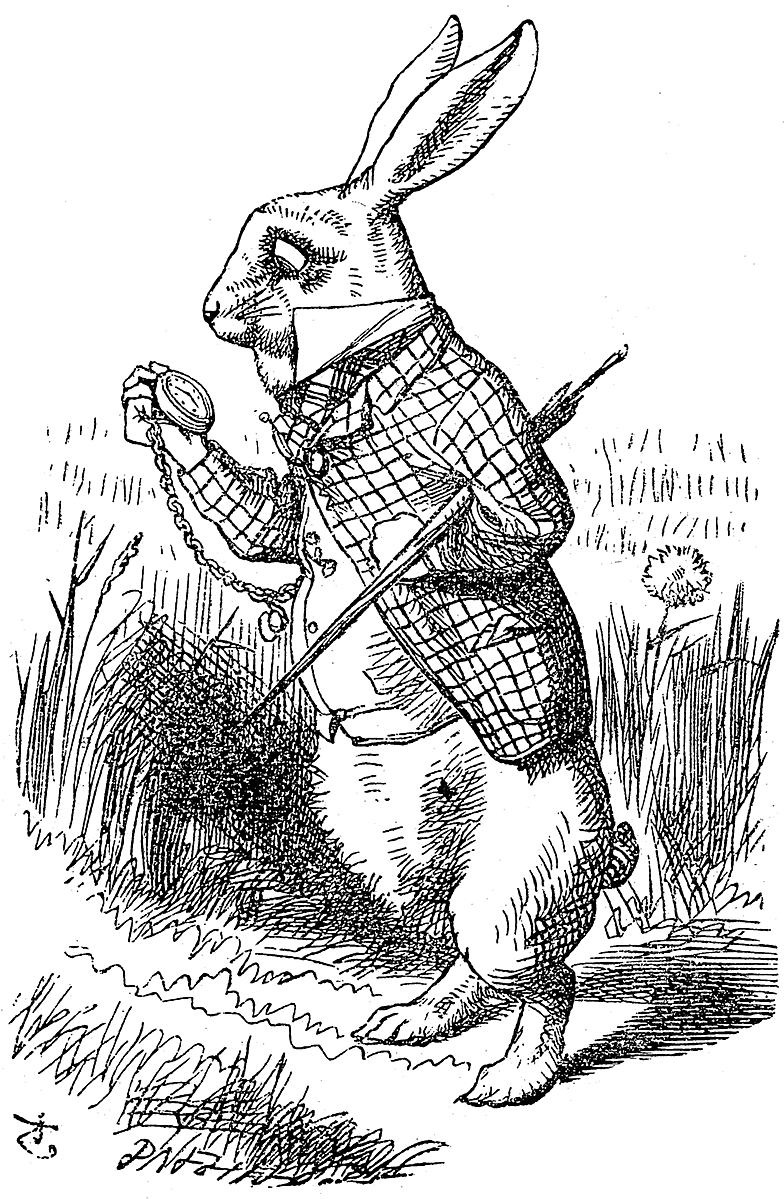
\includegraphics[width=\textwidth]{white-rabbit.png}
\end{column}

\end{columns}

\end{frame}

\begin{frame}[fragile]{Clever solution}

\begin{columns}[T]
  \begin{column}{.58\textwidth}

\fiboEq

\begin{lstlisting}[language=Haskell]
fibs :: [Integer]
fibs = 0 : 1 : zipWith (+)
                fibs (tail fibs)
\end{lstlisting}

\begin{lstlisting}[language=Haskell]
fib :: Word -> Integer
fib = genericIndex fibs
\end{lstlisting}

\end{column}

\begin{column}{.42\textwidth}
  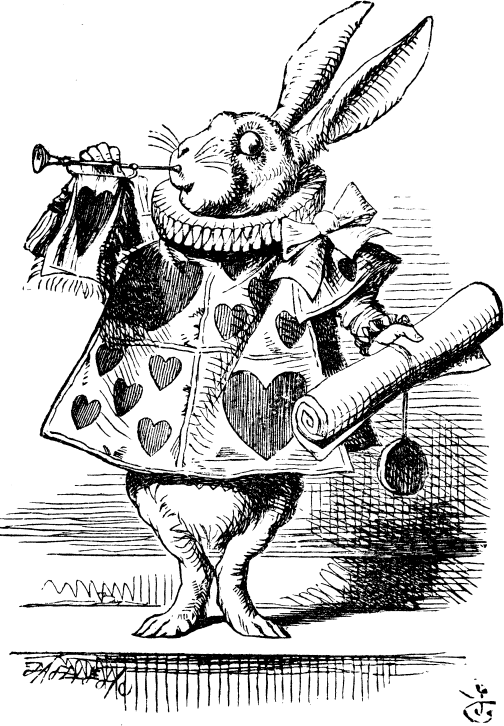
\includegraphics[width=\textwidth]{happy-rabbit.png}
\end{column}

\end{columns}

\end{frame}

\begin{frame}[fragile]{How it works? fibs = 0 : 1 : zipWith (+) fibs (tail fibs)}

\begin{columns}[T]
  \begin{column}{.7\textwidth}

\vspace{-3.5ex}

\begin{align*}
fibs       &= \textcolor{red}{0} : 1 : {\perp} \\
tail\ fibs &= \textcolor{red}{1} : {\perp} \\
\\
fibs       &= 0 : \textcolor{red}{1} : 1 : {\perp} \\
tail\ fibs &= 1 : \textcolor{red}{1} : {\perp} \\
\\
fibs       &= 0 : 1 : \textcolor{red}{1} : 2 : {\perp} \\
tail\ fibs &= 1 : 1 : \textcolor{red}{2} : {\perp} \\
\\
fibs       &= 0 : 1 : 1 : \textcolor{red}{2} : 3 : {\perp} \\
tail\ fibs &= 1 : 1 : 2 : \textcolor{red}{3} : {\perp} \\
\\
fibs       &= 0 : 1 : 1 : 2 : \textcolor{red}{3} : 5 : {\perp} \\
tail\ fibs &= 1 : 1 : 2 : 3 : \textcolor{red}{5} : {\perp} \\
\end{align*}

\end{column}

\begin{column}{.3\textwidth}
  \vspace{-2.0ex}
  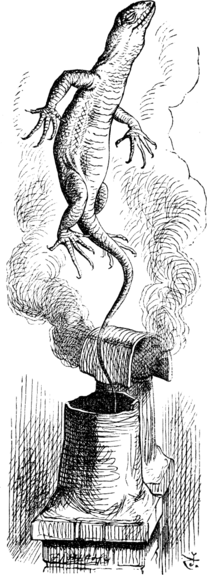
\includegraphics[width=\textwidth]{tail.png}
\end{column}

\end{columns}

\end{frame}

\begin{frame}[fragile]{Foobonacci numbers: 0, 1, 1, 3, 5, 11, 21, 43, 85, 171\dots}

$$
\mathcal{F}_n = \begin{cases}
n, & n < 2, \\
\mathcal{F}_{n-1} + \textcolor{red}{2}\mathcal{F}_{n-2}, & \text{otherwise}.
\end{cases}
$$

\begin{lstlisting}[language=Haskell]
foos :: [Integer]
foos = 0 : 1 : zipWith (\a b -> a+2*b) foos (tail foos)
\end{lstlisting}

\begin{lstlisting}[language=Haskell]
> take 10 foos
[0,1,2,5,12,29,70,169,408,985]
\end{lstlisting}

\begin{lstlisting}[language=Haskell]
foos :: [Integer]
foos = 0 : 1 : zipWith (\a b -> 2*a+b) foos (tail foos)
\end{lstlisting}

\end{frame}

\begin{frame}[fragile]{Barbonacci numbers: 0, 1, 2, 4, 11, 25, 59, 142, 335, 796\dots}

$$
B_n = \begin{cases}
n, & n < 3, \\
B_{n-1} + \textcolor{red}{2}B_{n-2} \textcolor{red}{{}+ 3B_{n-3}}, & \text{otherwise}.
\end{cases}
$$

\begin{lstlisting}[language=Haskell]
bars :: [Integer]
bars = 0 : 1 : 2 : zipWith3 (\a b c -> 3*a+2*b+c)
                    bars (tail bars) (drop 2 bars)
\end{lstlisting}

\begin{lstlisting}[language=Haskell]
bar :: Word -> Integer
bar n
  | n < 3     = toInteger n
  | otherwise = bar (n-1) + 2 * bar (n-2) + 3 * bar (n-3)
\end{lstlisting}

\end{frame}

\begin{frame}[fragile]{Catalan numbers: 1, 1, 2, 5, 14, 42, 132, 429, 1430, 4862\dots}

\begin{columns}[T]
  \begin{column}{.42\textwidth}

\centerline{Richard P. Stanley,}
\centerline{
  {\em Catalan numbers,}
  CUP, 2015
}

\def\redL{\textcolor{red}{(}}
\def\redR{\textcolor{red}{)}}
\def\greenL{\textcolor{green}{(}}
\def\greenR{\textcolor{green}{)}}
\def\blueL{\textcolor{blue}{(}}
\def\blueR{\textcolor{blue}{)}}

\begin{align*}
C_0 = 1  \\
C_1 = 1 & \qquad
  \redL \redR
  \\
C_2 = 2 & \qquad
  \redL\greenL\greenR\redR
  \quad \phantom{()}
  \redL\redR\greenL\greenR
  \\
C_3 = 5 & \qquad
  \redL\greenL\blueL\blueR\greenR\redR
  \quad
  \redL\greenL\greenR\redR\blueL\blueR
  \quad
  \redL\redR\greenL\blueL\blueR\greenR
  \\
  & \qquad
  \redL\greenL\greenR\blueL\blueR\redR
  \quad
  \redL\redR\greenL\greenR\blueL\blueR
\end{align*}

\vspace{-3ex}

\catalanEq

\end{column}

\begin{column}{.58\textwidth}
  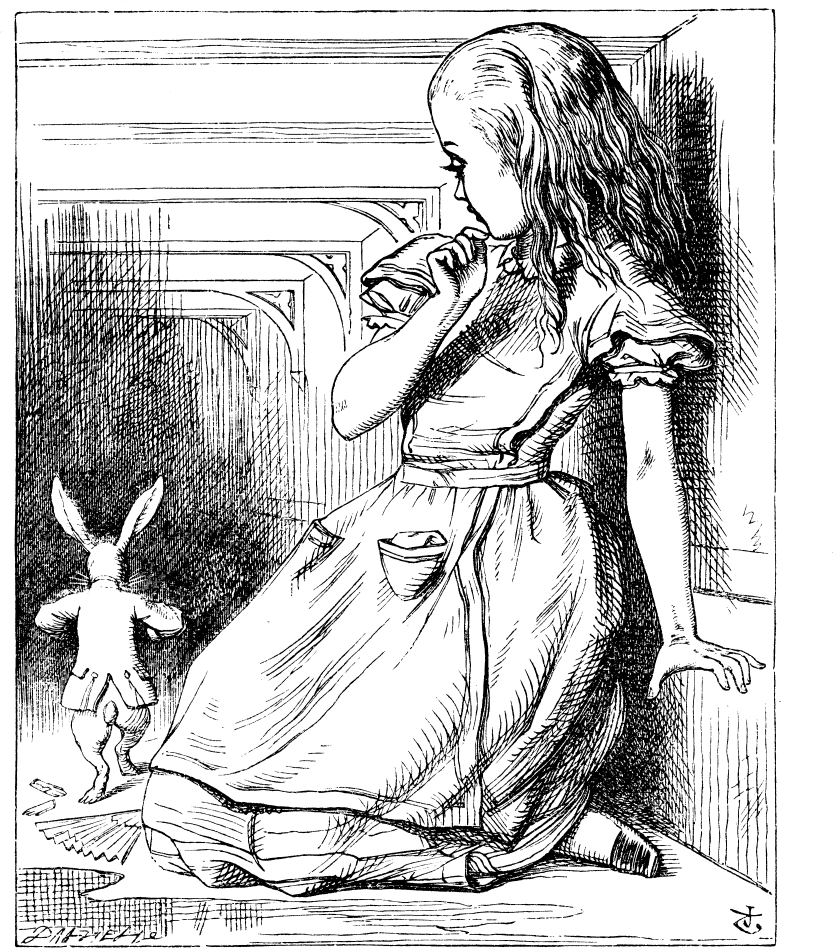
\includegraphics[width=\textwidth]{alice-and-rabbit.png}
\end{column}

\end{columns}

\end{frame}

\begin{frame}[fragile]{Very clever and not so clever solutions}

\catalanEq

\begin{lstlisting}[language=Haskell]
cat :: Word -> Integer
cat 0 = 1
cat n = sum $ map (\k -> cat k * cat (n-k-1)) [0..n-1]
\end{lstlisting}

\begin{lstlisting}[language=Haskell]
cats :: [Integer]
cats = 1 : map (\xs -> sum $ zipWith (*) xs (reverse xs))
               (tail $ inits cats)
\end{lstlisting}

\begin{lstlisting}[language=Haskell]
cats :: [Integer]
cats = 1 : map (\n -> sum $
  map (\k -> cats !! k * cats !! (n-k-1)) [0..n-1]) [1..]
\end{lstlisting}

\end{frame}

\begin{frame}[fragile]{Dynamic programming}

\begin{problem}
Alice is travelling over a one-dimensional chess board,
starting from the origin.
The Black Queen can move Alice
by 1, 4, 9, 16\dots cells, but only ahead.
Each cell $n$ contains $f(n)$ cakes.
For a given $N$ find
the maximum number of cakes $V(N)$, which Alice can collect
on her way to $N^{th}$ cell.
\end{problem}

\centerline{\textcolor{red}{
Through the looking-glass
a number of cakes may be negative!
}
}

\begin{columns}[T]
  \begin{column}{.5\textwidth}

  \begin{align*}
  V(0) &= f(0) \\
  V(n) &= f(n) + \max_{1 \le k \le \sqrt{n}} V(n - k^2)
  \end{align*}

\end{column}

\begin{column}{.5\textwidth}
  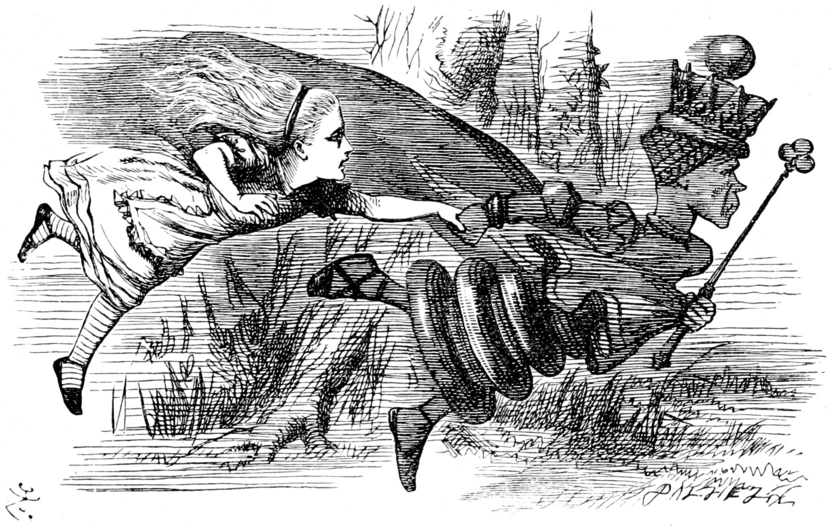
\includegraphics[width=1.13\textwidth]{alice-and-queen.png}
\end{column}

\end{columns}


\end{frame}

\begin{frame}[fragile]{Vectors to the rescue}

\begin{lstlisting}[language=Haskell]
fibs :: [Integer]
fibs = 0 : 1 : zipWith (+) fibs (tail fibs)
\end{lstlisting}

\begin{lstlisting}[language=Haskell]
fibs :: [Integer]
fibs = map (\n -> if n < 2
                  then toInteger n
                  else fibs !! (n-1) + fibs !! (n-2))
           [0..]
\end{lstlisting}

\begin{lstlisting}[language=Haskell]
import qualified Data.Vector as V
fibs :: V.Vector Integer
fibs = V.generate 100 $ \n ->
  if n < 2
  then toInteger n
  else fibs V.! (n-1) + fibs V.! (n-2)
\end{lstlisting}

\end{frame}

\begin{frame}[fragile]{Between lists and vectors}

  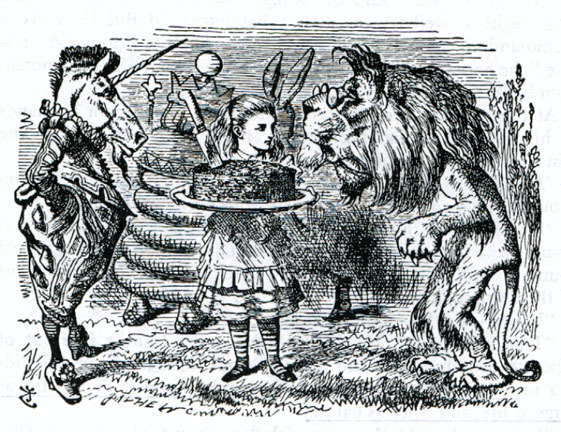
\includegraphics[width=1.03\textwidth]{lion-and-unicorn.png}

\end{frame}

\begin{frame}[fragile]{Lazy binary tree}

\begin{columns}[T]
  \begin{column}{.63\textwidth}

$$\xymatrix@C-2.1pc{
     &      &      & 0    & 1 \ar[dll]\ar[dr]   &      &      &      \\
     &      & 10 \ar[dl]\ar[dr]  &      &      & 11 \ar[dl]\ar[dr]   &      &      \\
     & 100 \ar[dl]\ar[d]  &      & 101 \ar[dl]\ar[d]  & 110 \ar[d]\ar[dr]  &      & 111 \ar[d]\ar[dr]  &      \\
1000 & 1001 & 1010 & 1011 & 1100 & 1101 & 1110 & 1111 \\
}$$

\begin{lstlisting}[language=Haskell]
data Tree a = Tree (Tree a) a (Tree a)
\end{lstlisting}

\end{column}

\begin{column}{.37\textwidth}
  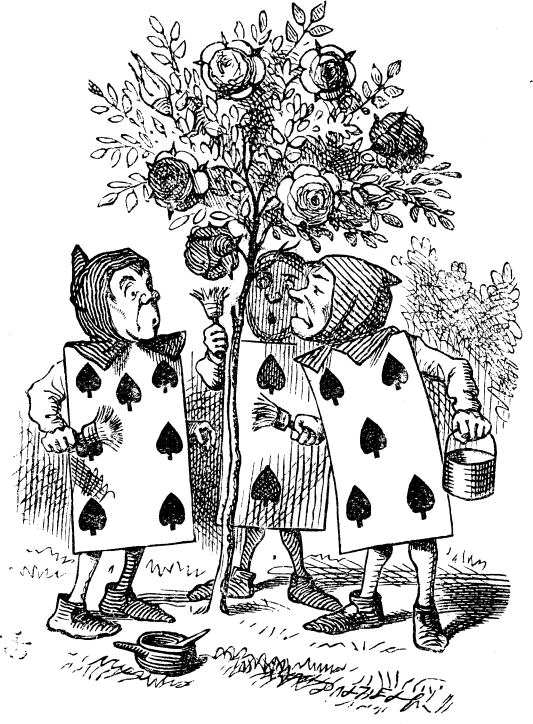
\includegraphics[width=1.18\textwidth]{gardeners.png}
\end{column}

\end{columns}

\end{frame}

\begin{frame}[fragile]{Lazy binary tree}

\begin{lstlisting}[language=Haskell]
data Tree a = Tree (Tree a) a (Tree a)
\end{lstlisting}

\begin{lstlisting}[language=Haskell]
tabulate :: (Word -> a) -> (a, Tree a)
tabulate f = (f 0, go 1) where
  go n = Tree (go (2 * n)) (f n) (go (2 * n + 1))
\end{lstlisting}

\begin{lstlisting}[language=Haskell]
index :: (a, Tree a) -> Word -> a
index (z, _) 0 = z
index (_, tree) n = go tree n where
  go (Tree _ m _) 1 = m
  go (Tree l _ r) k =
    go (if even n then l else r) (k `quot` 2)
\end{lstlisting}

\begin{lstlisting}[language=Haskell]
fib :: Word -> Integer
fib n = if n<2 then toInteger n else fib'(n-1) + fib'(n-2)

fib' :: Word -> Integer
fib' n = index (tabulate fib) n
\end{lstlisting}

\end{frame}

\begin{frame}[fragile]{Fixed-point combinator}

\begin{lstlisting}[language=Haskell]
fix :: (a -> a) -> a
fix f = f (fix f)
\end{lstlisting}

\begin{lstlisting}[language=Haskell]
fibF :: (Word -> Integer) -> Word -> Integer
fibF f n = if n<2 then toInteger n else f (n-1) + f (n-2)
\end{lstlisting}

\begin{lstlisting}[language=Haskell]
tabulate :: (Word -> a) -> (a, Tree a)
tabulate f = (f 0, go 1) where
  go n = Tree (go (2*n)) (f n) (go (2*n+1))
\end{lstlisting}

\begin{lstlisting}[language=Haskell]
tabulateFix :: ((Word -> a) -> Word -> a) -> (a, Tree a)
tabulateFix f = res where
  res = (f 0, go 1)
  go n = Tree (go (2*n)) (f (index res) n) (go (2*n+1))
\end{lstlisting}

\end{frame}

\begin{frame}[fragile]{Chimera = Vector (Vector a)}

\begin{columns}[T]
  \begin{column}{.59\textwidth}

\def\red#1{\textcolor{red}{#1}}
\def\green#1{\textcolor{green}{#1}}
\def\blue#1{\textcolor{blue}{#1}}

$$
\!\!\!\!\!\!
\!\!\!
\xymatrix@C-2.1pc{
     &      &      & 0    & 1 \ar[dll]\ar[dr]   &      &      &      \\
     &      & \red{10} \ar[dl]\ar[dr]  &      &      & \red{11} \ar[dl]\ar[dr]   &      &      \\
     & \green{100} \ar[dl]\ar[d]  &      & \green{101} \ar[dl]\ar[d]  & \green{110} \ar[d]\ar[dr]  &      & \green{111} \ar[d]\ar[dr]  &      \\
\blue{1000} & \blue{1001} & \blue{1010} & \blue{1011} & \blue{1100} & \blue{1101} & \blue{1110} & \blue{1111} \\
}
$$

\begin{multline*}
\!\!
\bigl[
[0],
[1],
[10, 11],
[100, 101, 110, 111], \\
\!\!\! \!\!\! \!\!\!
[1000, 1001, 1010, 1011, 1100, 1101, 1110, 1111]
\bigr]
\end{multline*}

\end{column}

\begin{column}{.4\textwidth}
  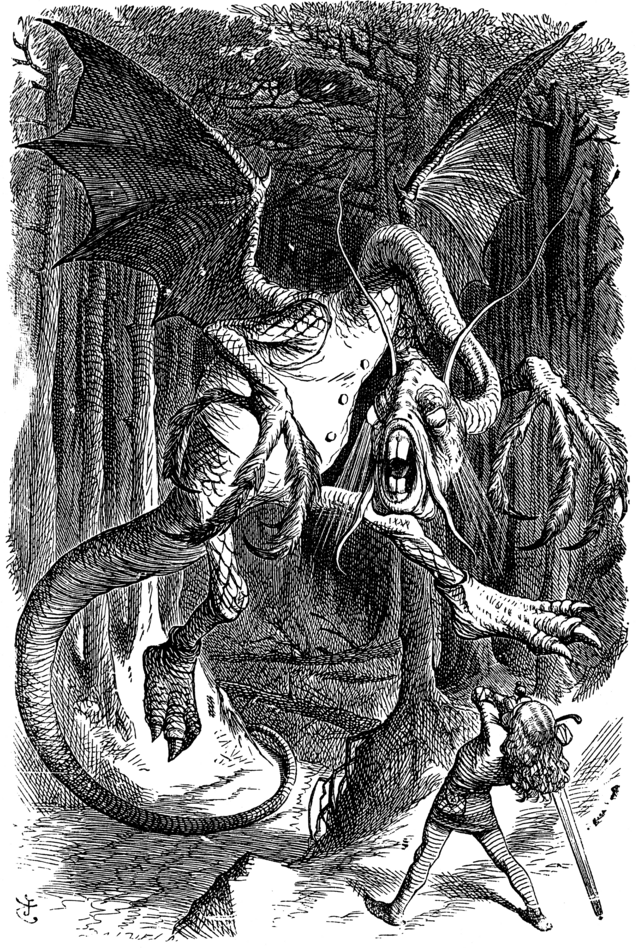
\includegraphics[width=1.18\textwidth]{jabberwocky.png}
\end{column}

\end{columns}

\end{frame}

\begin{frame}[fragile]{Magic and its exposure}

\begin{columns}[T]
  \begin{column}{.55\textwidth}

\textcolor{blue}{\tt newtype }%
{\tt Chimera a =}%
\par
{\tt ~~Chimera (}%
\textcolor{red}{\tt Vector }%
{\tt (}%
\textcolor{green}{\tt Vector }%
{\tt a))}

\bigskip

A boxed outer
\textcolor{red}{\tt Vector}
points to 65~inner
\textcolor{green}{\tt Vector}s
of growing sizes
$$
1, 1, 2, 2^2, 2^3, \ldots, 2^{62}, 2^{63}.
$$

\fbox{$f(0)$} ~
\fbox{$f(1)$} ~
\fbox{$f(2)$}\fbox{$f(3)$}
\vspace{1ex}\par
\hfill
\fbox{$f(4)$}\fbox{$f(5)$}\fbox{$f(6)$}\fbox{$f(7)$}

\bigskip

Inner
\textcolor{green}{\tt Vector}s
are allocated on-demand,
resembling
dynamic arrays in imperative languages,
but caught in amber.

\end{column}

\begin{column}{.45\textwidth}
  \vspace{-2ex}
  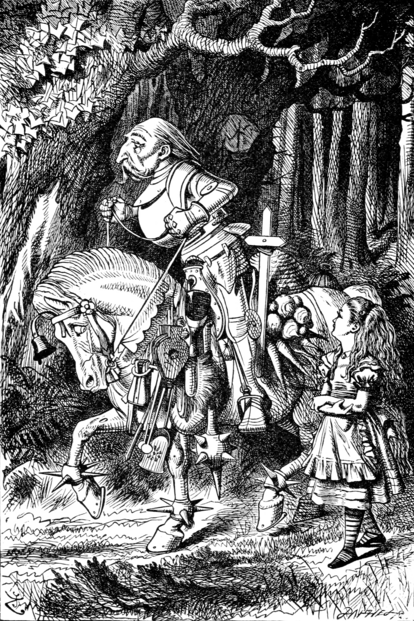
\includegraphics[width=1.15\textwidth]{white-knight.png}
\end{column}

\end{columns}

\end{frame}

\begin{frame}[fragile]{Bit tweedling}

\begin{columns}[T]
  \begin{column}{.65\textwidth}

\begin{lstlisting}[language=Haskell]
import Data.Vector (Vector, (!))
import qualified Data.Vector as V

data Chimera a =
  Chimera (Vector (Vector a))
\end{lstlisting}

\begin{lstlisting}[language=Haskell]
tabulate :: (Word -> a) -> Chimera a
tabulate f = Chimera $ V.singleton (f 0) `V.cons`
  V.generate 64 (\k -> V.generate (2^k) (f . (+ 2^k)))
\end{lstlisting}

\begin{lstlisting}[language=Haskell]
index :: Chimera a -> Word -> a
index (Chimera xss) 0 = xss ! 0 ! 0
index (Chimera xss) n = xss ! (64-clz) ! (n - 2^(63-clz))
  where
    clz = countLeadingZeros n
\end{lstlisting}

\end{column}

\begin{column}{.45\textwidth}
  \vspace{-3ex}
  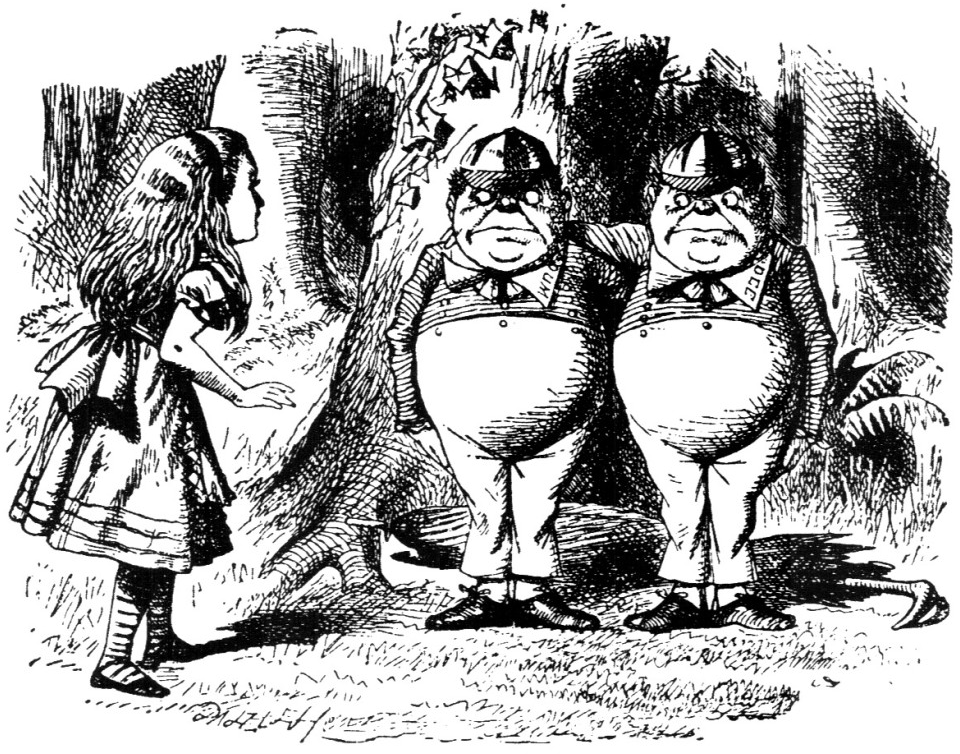
\includegraphics[width=1.07\textwidth]{tweedledum.png}
\end{column}

\end{columns}

\end{frame}

\begin{frame}[fragile]{Representable functor for {\tt Word}}

\begin{columns}[T]
  \begin{column}{.6\textwidth}

$$
\mathrm{Chimera}(a) \cong \mathrm{Hom}(\mathrm{Word}, a)
$$

$$
\mathrm{Chimera} \cong \mathrm{Hom}(\mathrm{Word}, \cdot)
$$

\begin{lstlisting}[language=Haskell]
import Data.Functor.Rep
instance Representable Chimera where
  type Rep Chimera = Word
  tabulate = tabulate
  index = index
\end{lstlisting}

GHC can derive
{\tt Functor},
{\tt Foldable},
{\tt Traversable}.

And {\tt adjunctions} package is able to provide
{\tt Applicative},
{\tt Monad},
{\tt MonadFix},
{\tt MonadZip},
{\tt Distributive}.

\end{column}

\begin{column}{.4\textwidth}
  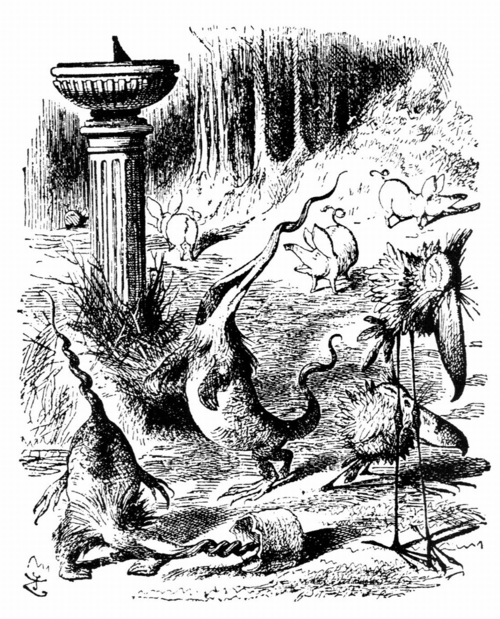
\includegraphics[width=1.2\textwidth]{zoo.png}
\end{column}

\end{columns}

\end{frame}

% \begin{frame}[fragile]{Random streams}

% \begin{lstlisting}[language=Haskell]
% tabulateM :: Monad m => (Word -> m a) -> m (Chimera a)
% \end{lstlisting}

% \begin{lstlisting}[language=Haskell]
% instance Arbitrary a => Arbitrary (Chimera a) where
%   arbitrary = tabulateM (const arbitrary)
% \end{lstlisting}

% \textcolor{green}{\bf Good monads:}
% {\tt Identity},
% {\tt Reader}, lazy {\tt Writer}, lazy {\tt State}.

% \medskip

% \textcolor{red}{\bf Bad monads:}
% strict {\tt State}, {\tt IO}.

% \end{frame}

\begin{frame}[fragile]{Cellular automata 1D}

{\bf Rule 90.}
An infinite in both directions line of cells, each being dead ({\tt False}) or alive ({\tt True}). If two neighbours of a cell are equal, it becomes dead at the next step, otherwise alive.

\begin{lstlisting}[language=Haskell]
step :: (Int -> Bool) -> (Int -> Bool)
step current = \n -> current (n - 1) /= current (n + 1)
\end{lstlisting}

\begin{lstlisting}[language=Haskell]
step :: Chimera Bool -> Chimera Bool
step current = tabulate $ \n ->
  current `index` (n - 1) /= current `index` (n + 1)
\end{lstlisting}

Use continuous mappings:

\begin{lstlisting}[language=Haskell]
>>> map intToWord [-5..5]
[9,7,5,3,1,0,2,4,6,8,10]
>>> map wordToInt [0..10]
[0,-1,1,-2,2,-3,3,-4,4,-5,5]
\end{lstlisting}

\end{frame}

\begin{frame}[fragile]{Cellular automata 2D}

{\bf Conway's Game of Life.}
An infinite in all directions plane of cells.
If a live cell has 2 or 3 neighbours, it remains alive at the next step,
otherwise dies. An empty cell with exactly 3 neighbours becomes alive at the next step.

\begin{lstlisting}[language=Haskell]
step :: (Int -> Int -> Bool) -> (Int -> Int -> Bool)
\end{lstlisting}

\begin{lstlisting}[language=Haskell]
step :: (Word -> Word -> Bool) -> (Word -> Word -> Bool)
\end{lstlisting}

\begin{columns}[T]
  \begin{column}{.52\textwidth}

Interleave binary coordinate values:

\begin{lstlisting}[language=Haskell]
> toZCurve 0b0000 0b1111
0b01010101
> fromZCurve 0b010101010
(0b0000, 0b1111)
\end{lstlisting}

\end{column}

\begin{column}{.48\textwidth}
  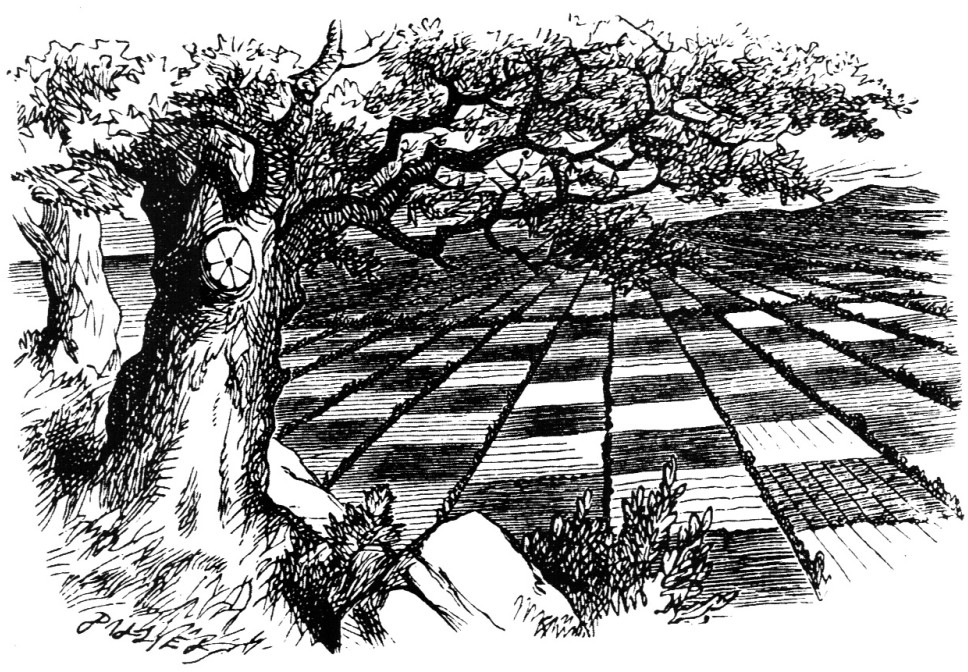
\includegraphics[width=1.11\textwidth]{chess.png}
\end{column}

\end{columns}

\end{frame}

\begin{frame}[fragile]{Unboxed vectors and predicates}

\begin{lstlisting}[language=Haskell]
newtype Chimera v a = Chimera (Vector (v a))

type UChimera = Chimera Data.Vector.Unboxed.Vector
\end{lstlisting}

\begin{lstlisting}[language=Haskell]
isPrime :: Word -> Bool
isPrime n = n>1 && and [n `rem` d /= 0 | d <- [2..n-1]]
\end{lstlisting}

\begin{columns}[T]
  \begin{column}{.45\textwidth}

Use {\tt bitvec} package to pack booleans densely:

\begin{lstlisting}[language=Haskell]
import Data.Bit

isPrime' :: UChimera Bit
isPrime' = tabulate
  (Bit . isPrime)
\end{lstlisting}

\end{column}

\begin{column}{.55\textwidth}
  \vspace{1.6ex}

  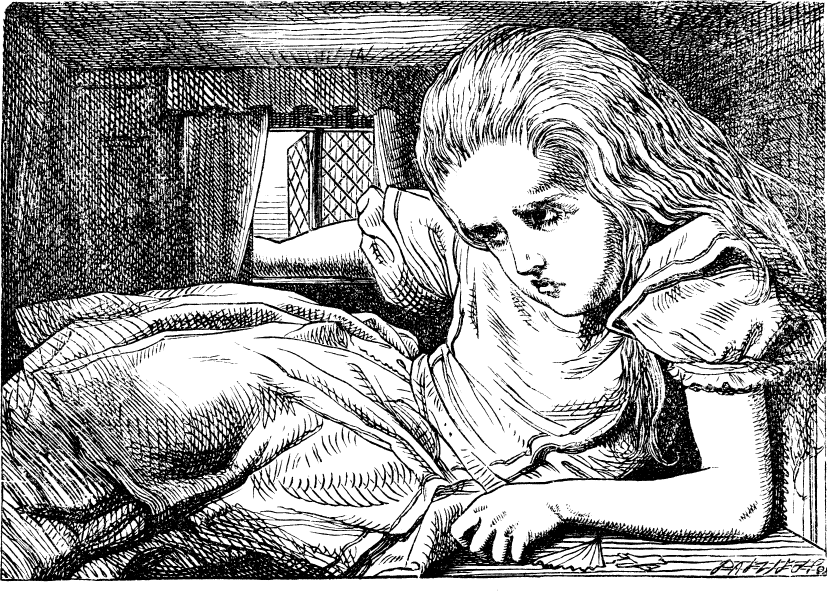
\includegraphics[width=1.11\textwidth]{boxed-alice.png}
\end{column}

\end{columns}

\end{frame}

\begin{frame}

\begin{columns}[T]
  \begin{column}{.51\textwidth}

\bigskip
\bigskip
\bigskip
\bigskip

\par \faAt\ andrew.lelechenko@gmail.com

\bigskip

\par \faGithub\ github.com/Bodigrim/chimera

\bigskip

\par \faGithub\ github.com/Bodigrim/my-talks

\bigskip
\bigskip
\bigskip

\centerline{\Huge\bf Thank you!}

\end{column}

\begin{column}{.5\textwidth}
  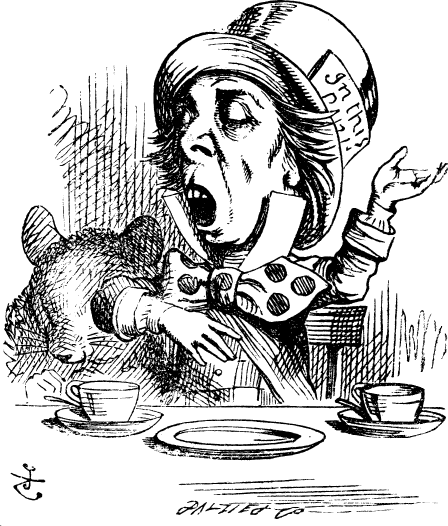
\includegraphics[width=1.1\textwidth]{mad-hatter.png}

  {\hfill \tiny Illustrations by Sir John Tenniel}
\end{column}

\end{columns}

\end{frame}

\end{document}
